\sectioncounter{16}
\section{同角三角函数间基本关系与诱导公式}

\subsection{知识梳理}
同角三角函数有两个常用的基本关系式
\[\sin^2 x+ \cos^2 x= 1,\quad 
    \tan x= \frac{\sin x}{\cos x}.\]
前一个式子等价于勾股定理, 且由该式可知
\[(\sin x\pm \cos x)^2= 1\pm 2\sin x\cos x.\]
后一个式子也可以看作正切的定义.

凡正弦、余弦的二次式, 均可以用正切函数表示, 例如:
\[\sin x\cos x+ \cos^2 x
    = \frac{\sin x\cos x+ \cos^2 x}{\sin^2 x+ \cos^2 x}
    = \frac{\tan x+ 1}{\tan^2 x+ 1}.\]
与此类似的还有
\[\frac{\sin x+2\cos x}{3\sin x-\cos x}
    = \frac{\dfrac{\sin x}{\cos x}+2}{\dfrac{3\sin x}{\cos x}-1}
    = \frac{\tan x+2}{3\tan x-1}.\]
这两种变形方法常用来解决正弦、余弦值和正切值的转化问题.

诱导公式指的是已知角加上 $90^\circ$ (或 $\dfrac{\pi}2$) 的整数倍后,
所得角与已知角的三角函数值的关系. 除了
\[\begin{gathered}
    \sin(360^\circ+x)= \sin x,\quad \cos(360^\circ+x)= \cos x\\
    \sin(180^\circ+x)= -\sin x,\quad \cos(180^\circ+x)= -\cos x,
\end{gathered}\]
常用的诱导公式还有
\[\begin{gathered}
    \sin(-x)= -\sin x,\quad \cos(-x)= \cos x,\\
    \sin(90^\circ-x)= \cos x,\quad \cos(90^\circ-x)= \sin x,\\
    \sin(180^\circ-x)= \sin x,\quad \cos(180^\circ-x)= -\cos x,
\end{gathered}\]
等等. 诱导公式的的合理性见下图:
\begin{center}
    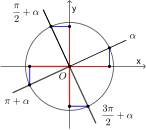
\includegraphics[scale=1.1]{2020-1225-1930-crop}
\end{center}

诱导公式的记忆口诀为: \myemph{奇变偶不变, 符号看象限},
其中的 ``奇偶'' 指所加 $90^\circ$ (或 $\dfrac{\pi}2$) 倍数的奇偶, 
``变'' 指函数名中正变余或余变正, ``象限''指把已知角视为锐角时所得角对应的象限, 而 ``符号'' 是此时原式的符号. 例如
\[\begin{gathered}
    \sin(2x-\pi)= -\sin2x,\quad \tan(x+180^\circ)= \tan x, \\
    \cos(3x-270^\circ)= -\sin 3x,\quad
    \sin\biggl(4x-\frac{\pi}2\biggr)= -\cos 4x.
\end{gathered}\]

诱导公式最基本的用途是将任意角的三角函数值化为锐角三角函数值, 例如
\[\begin{aligned}
    \sin1215^\circ
    &= \sin(3\cdot 360^\circ+ 135^\circ)= \sin135^\circ\\
    &= \sin(180^\circ- 45^\circ)= \sin45^\circ= \frac{\sqrt2}{2},\\
    \cos(-750^\circ)
    &= \cos(-2\cdot 360^\circ- 30^\circ)= \cos(-30^\circ)\\
    &= \cos30^\circ= \frac{\sqrt3}{2},\\
    \tan660^\circ
    &= \tan(2\cdot 360^\circ- 60^\circ)= \tan(-60^\circ)\\
    &= -\tan60^\circ= -\sqrt3.
\end{aligned}\]
利用正切函数为奇函数且最小正周期为 $180^\circ$, 最后一式也可以变形如下:
\[\begin{aligned}
    \tan660^\circ
    &= \tan(3\cdot 180^\circ+ 120^\circ)= \tan120^\circ\\
    &= \tan(180^\circ-60^\circ)= -\tan60^\circ= -\sqrt3.
\end{aligned}\]
    
\lianxi
\begin{exercise}
    若 $\cos\alpha =\dfrac35$, 
    $\alpha\in\Bigl(-\dfrac{\pi}2,0\Bigr)$, 求 $\tan\alpha$ 的值.
\end{exercise}
\beginsolution
    由 $|\sin\alpha|= \dfrac45$ 和 $\sin\alpha< 0$ 知, 
    \mymarginpar{也可以先画三角函数线, 由直角三角形三边的比例关系写出 $|\tan\alpha|$.}
    $\sin\alpha= -\dfrac45$.
\endsolution

\begin{exercise}
    若 $\tan\alpha =3$, 求 $\dfrac{3\sin\alpha- \cos\alpha}{\sin\alpha+ \cos\alpha}$ 的值. 
\end{exercise}
\beginsolution
    方法一: 由 $\tan\alpha =3$ 知 $\sin\alpha= 3\cos\alpha$, 所以
    \[\frac{3\sin\alpha- \cos\alpha}{\sin\alpha+ \cos\alpha}
    = \frac{3\cdot 3\cos\alpha- \cos\alpha}{3\cos\alpha+ \cos\alpha}
    = 2.\]

    方法二: 分子、分母同除以 $\cos\alpha$, 
    \mymarginpar{方法一是更通用的解法, 方法二是针对此类题的特殊解法.}
    \[\frac{3\sin\alpha- \cos\alpha}{\sin\alpha+ \cos\alpha}
    = \frac{3\tan\alpha- 1}{\tan\alpha+ 1}
    = 2.\]
\endsolution

\begin{exercise}
    若 $\alpha$ 是第一象限角, 化简: $\tan\alpha\cdot \sqrt{\dfrac1{\sin^2\alpha}- 1}$.
\end{exercise}
\beginsolution
    原式 $= \tan\alpha\cdot \sqrt{\dfrac{\cos^2\alpha}{\sin^2\alpha}}
    = \tan\alpha\cdot \dfrac{\cos\alpha}{\sin\alpha}
    = 1$.
\endsolution

\begin{exercise}
    化简: $\sin(\pi-2)+\sin(3\pi+2)$.
\end{exercise}
\beginsolution
    原式 $= \sin2+\sin(\pi+2)= \sin2- \sin2= 0$.
\endsolution

\begin{exercise}
    如果 $\cos\alpha =\dfrac15$, 且 $\alpha$ 是第四象限角,
    求 $\cos\biggl(\alpha+\dfrac{\pi}2\biggr)$ 的值.
\end{exercise}
\beginsolution
    $\cos\biggl(\alpha+\dfrac{\pi}2\biggr)= \sin\alpha
    = -\biggl(-\dfrac{2\sqrt6}5\biggr)
    = \dfrac{2\sqrt6}5$.
\endsolution

\subsection{要点导学\quad 各个击破}
\subsubsection{利用同角三角函数关系求值}
\begin{example}
    已知 $\sin x= \dfrac5{13}$, 求 $\cos x$ 与 $\tan x$ 的值.
\end{example}
\beginsolution
    若 $x$ 在第一象限, 则
    \[\cos x= \frac{12}{13},\quad
        \tan x= \frac{5}{12};\]
    若 $x$ 在第二象限, 则
    \[\cos x= -\frac{12}{13},\quad
        \tan x= -\frac{5}{12}.\]
\endsolution

\begin{example}
    已知 $\sin\alpha = -3\cos\alpha$, 求下列各式的值:
    
    (1) $\dfrac{\sin^2 \alpha+ 2\cos^2 \alpha}{ 
      \sin^2 \alpha+ \sin\alpha \cos\alpha}$;\qquad 
    (2) $1+\sin\alpha \cos\alpha$.
\end{example}
\beginsolution
    (1) 方法一: 由已知, $\tan\alpha= \dfrac{\sin\alpha}{\cos\alpha}= -3$, 所以
    \[\text{原式}= \frac{\tan^2 \alpha+ 2}{ 
        \tan^2 \alpha+ \tan\alpha}
        = \frac{(-3)^2+2}{(-3)^2-3}
        = \frac{11}{6}.\]
    
    方法二: 直接将 $\sin\alpha = -3\cos\alpha$ 代入,
    \[\text{原式}= \frac{(-3\cos\alpha)^2+ 2\cos^2\alpha}{ 
        (-3\cos\alpha)^2+ (-3\cos\alpha)\cdot\cos\alpha}
        = \frac{(-3)^2+2}{(-3)^2-3}
        = \frac{11}{6}.\]
    
    (2) 因为 $\sin\alpha = -3\cos\alpha$, 所以 
    \[\sin^2\alpha+ \cos^2\alpha= (-3\cos\alpha)^2+ \cos^2\alpha= 1,\]
    即 $\cos^2\alpha= \dfrac1{10}$, 故
    \[1+\sin\alpha \cos\alpha
        = 1- 3\cos^2\alpha= \frac{7}{10}.\]
\endsolution

\lianxi
\begin{exercise}[s]
    已知 $\tan(\pi-\alpha)= \dfrac12$, 那么 $\dfrac{\sin\alpha+ 
      \cos\alpha}{2\sin\alpha- \cos\alpha}$ 的值.
\end{exercise}
\beginsolution
    由已知, $-\tan\alpha= \dfrac12$ 即 $\tan\alpha= -\dfrac12$, 所以
    \[\text{原式}= \frac{\tan\alpha+1}{2\tan\alpha-1}
        = \frac{-\dfrac12+1}{2\Bigl(-\dfrac12\Bigr)-1}
        = -\frac14.\]
\endsolution

\subsubsection{$\sin\theta\pm\cos \theta$ 与 $\sin\theta\cos\theta$ 的关系}
\begin{example}
    已知 $0<\theta<\pi$ 且 $\sin\theta+\cos\theta= -\dfrac15$,
    求 $\tan\theta$ 的值.
\end{example}
\beginsolution
    由已知, $\sin\theta>0$ 且
    \[\left\{\!\!\begin{array}{l}
        \sin\theta+\cos\theta= -\dfrac15,\\
        \sin^2\theta+ \cos^2\theta= 1,
    \end{array}\right.\ \text{解得}\ 
    \left\{\!\!\begin{array}{l}
        \sin\theta= \dfrac35,\\
        \cos\theta= -\dfrac45,
    \end{array}\right.\]
    所以 $\tan\theta= \dfrac{\sin\theta}{\cos\theta}= -\dfrac34$.
\endsolution

\begin{example}
    已知 $\sin\alpha+ \cos\alpha = \dfrac34$ 且 $\dfrac{\pi}4 <\alpha < \dfrac{\pi}2$, 求 $\cos\alpha -\sin\alpha$ 的值.
\end{example}
\beginsolution
    因为 $\sin\alpha+ \cos\alpha = \dfrac34$ 且
    \[(\sin\alpha+\cos\alpha)^2+ (\sin\alpha-\cos\alpha)^2= 2,\]
    所以 $|\cos\alpha-\sin\alpha|= \dfrac{\sqrt7}4$. 再由 $\dfrac{\pi}4 <\alpha < \dfrac{\pi}2$ 知 $\cos\alpha< \sin\alpha$, 故 
    \[\cos\alpha-\sin\alpha= -\dfrac{\sqrt7}4.\]
\endsolution

\lianxi
\begin{exercise}[s]
    已知 $\sin\theta+ 2\cos\theta= 2$, 求 $\tan\theta$ 的值.
\end{exercise}
\beginsolution
    结合 $\sin^2\theta+ \cos^2\theta= 1$ 可解得
    \[\left\{\!\!\begin{array}{l}
        \sin\theta= \frac45,\\[6pt]
        \cos\theta= \frac35,
    \end{array}\right.\ \text{或}\ 
    \left\{\!\!\begin{array}{l}
        \sin\theta= 0,\\
        \cos\theta= 1.
    \end{array}\right.\]
    所以 $\tan\theta= \dfrac{\sin\theta}{\cos\theta}= \dfrac43$ 或 $0$.
\endsolution

\subsubsection{利用诱导公式进行化简与求值}
\begin{example}
    (1) 已知 $\cos(\pi+\alpha)= -\dfrac12$, $\dfrac{3\pi}2< \alpha< 2\pi$, 
    求 $\sin(2\pi-\alpha)$ 的值;
    
    (2) 已知 $\dfrac{1+2\sin(\pi+\theta)}{2-\sin(-\theta)}= \dfrac{11}7$, 
    求 $\tan(\theta+\pi)\cos(\theta-\pi)$ 的值.
\end{example}
\beginsolution
    (1) 由 $\cos(\pi+\alpha)= -\dfrac12$ 知
    \[-\cos\alpha= -\dfrac12\ \text{即}\ 
    \cos\alpha= \dfrac12.\]
    因为 $\dfrac{3\pi}2< \alpha< 2\pi$, 
    \mymarginpar{由 $\cos\alpha= \dfrac12$ 和 $\dfrac{3\pi}2< \alpha< 2\pi$ 可解出 $\alpha= \dfrac{5\pi}3$.}
    所以 $\sin\alpha= -\dfrac{\sqrt3}2$,
    \[\sin(2\pi-\alpha)= -\sin\alpha= \frac{\sqrt3}{2}.\]

    (2) 由已知,
    \[\dfrac{1-2\sin\theta}{2+\sin\theta}= \dfrac{11}7,
        \quad\text{解得}\quad
        \sin\theta= -\frac35,\]
    所以
    \[\tan(\theta+\pi)\cos(\theta-\pi)
        = \tan\theta(-\cos\theta)
        = -\sin\theta= \frac35.\]
\endsolution

\begin{example}
    已知 $\cos(75^\circ+\alpha)= \dfrac13$, 且 $\alpha\in[-180^\circ,-90^\circ]$, 求 $\cos(15^\circ-\alpha)+ \sin(\alpha-15^\circ)$ 的值.
\end{example}
\beginsolution
    本题宜用 ``换元法'' 来解. 设 $75^\circ+\alpha= \beta$, 
    \mymarginpar{若题中 $\alpha$ 改为第三象限角, 则答案不变, 因为此时 $\beta$ 在第二、三象限或第三、四象限, 而由 $\cos\beta> 0$ 知, $\beta$ 只能在第四象限.}
    则
    \[\beta\in[-105^\circ,-15^\circ],\ 
        \alpha= \beta- 75^\circ\ \text{且}\ 
        \cos\beta= \frac13,\]
    因此 $\sin\beta= -\dfrac{2\sqrt2}3$. 而
    \[\begin{gathered}
        \cos(15^\circ-\alpha)= \cos(90^\circ- \beta)= \sin\beta,\\
        \sin(\alpha-15^\circ)= \sin(\beta- 90^\circ)= -\cos\beta,
    \end{gathered}\]
    代入所求式子知
    \[\cos(15^\circ-\alpha)+ \sin(\alpha-15^\circ)
        = \sin\beta- \cos\beta= -\frac{1+2\sqrt2}{3}.\]
\endsolution

\lianxi
\begin{exercise}
    已知 $\sin\biggl(\dfrac\pi6- \theta\biggr)=a$, 
    求 $\cos\biggl(\dfrac{2\pi}3-\theta\biggr)$ 的值.
\end{exercise}
\beginsolution
    设 $\dfrac\pi6- \theta= \varphi$, 则 $\theta= \dfrac\pi6- \varphi$ 且 $\sin\varphi= a$, 所以
    \[\cos\biggl(\dfrac{2\pi}3-\theta\biggr)
        = \cos\biggl(\frac\pi2+\varphi\biggr)
        = -\sin\varphi= -a.\]
\endsolution

\begin{exercise}
    已知 $\sin\biggl(x+\dfrac\pi6\biggr)= \dfrac13$, 
    求 $\sin\biggl(\dfrac{7\pi}6+x\biggr)+ 
      \cos^2\biggl(\dfrac{5\pi}6-x\biggr)$ 的值.
\end{exercise}
\beginsolution
    设 $x+\dfrac\pi6=y$, 则 $x=y-\dfrac\pi6$ 且 $\sin y= \dfrac13$, 所以
    \[\begin{aligned}
        \sin\biggl(\dfrac{7\pi}6+x\biggr)
        = \sin(\pi+y)= -\sin y= -\frac13,\\
        \cos^2\biggl(\dfrac{5\pi}6-x\biggr)
        = \cos^2(\pi-y)= \cos^2y= \frac89,
    \end{aligned}\]
    故
    \[\sin\biggl(\dfrac{7\pi}6+x\biggr)+ 
    \cos^2\biggl(\dfrac{5\pi}6-x\biggr)
        = -\frac13+ \frac89= \frac59.\]
\endsolution

\subsubsection{课堂评价}

\begin{exercise}
    求值: $\sin 585^\circ$, $\cos 495^\circ$, $\tan\dfrac{11\pi}4$.
\end{exercise}
\beginsolution
    利用诱导公式,
    \[\begin{aligned}
        \sin 585^\circ
        &= \sin (2\cdot360^\circ- 135^\circ)
         = -\sin 135^\circ\\
        &= -\sin45^\circ= -\frac{\sqrt2}{2},\\
        \cos 495^\circ
        &= \cos(360^\circ+ 135^\circ)= \cos135^\circ\\
        &= -\cos45^\circ= -\frac{\sqrt2}{2},\\
        \tan\dfrac{11\pi}4
        &= \tan\biggl(3\pi-\frac\pi4\biggr)
         = \tan\biggl(-\frac\pi4\biggr)\\
        &= -\tan\frac\pi4= -1.
    \end{aligned}\]
\endsolution

\begin{exercise}
    已知 $\sin\biggl(\dfrac{5\pi}2+ \alpha\biggr)= \dfrac15$, 
    求 $\cos\alpha$ 的值.
\end{exercise}
\beginsolution
    因为 
    \[\sin\biggl(\dfrac{5\pi}2+ \alpha\biggr)
        = \sin\biggl(\dfrac{\pi}2+ \alpha\biggr)
        = \cos\alpha,\]
    所以 $\cos\alpha= \frac15$.
\endsolution

\begin{exercise}
    设 $\alpha$ 是第三象限角, 若 $\tan\alpha =\dfrac5{12}$, 
    求 $\cos\alpha $ 的值.
\end{exercise}
\beginsolution
    画三角函数线知, $|\cos\alpha|= \dfrac{12}{13}$, 而 $\cos\alpha<0$, 所以 $\cos\alpha= -\dfrac{12}{13}$.
\endsolution

\begin{exercise}
    已知 $\tan\alpha =2$, 求 $\sin\alpha \cos\alpha$ 的值.
\end{exercise}
\beginsolution
    方法一: 直接变形,
    \[\sin\alpha \cos\alpha
        = \frac{\sin\alpha \cos\alpha}{\sin^2\alpha+ \cos^2\alpha}
        = \frac{\tan\alpha}{\tan^2\alpha+1}
        = \frac25.\]

    方法二: 由 $\tan\alpha =2$ 知 $\sin\alpha= 2\cos\alpha$, 则
    \[1= \sin^2\alpha+ \cos^2\alpha= 4\cos^2\alpha+ \cos^2\alpha,\]
    即 $\cos^2\alpha= \dfrac15$, 所以
    \[\sin\alpha \cos\alpha= 2\cos^2\alpha= \frac25.\]
\endsolution

\subsection{课后练习}
\begin{exercise}
    若 $\alpha$ 是钝角, 且 $\sin\alpha =\dfrac13$, 求 $\tan\alpha $ 的值.
\end{exercise}
\beginsolution
    画三角函数线知, $|\cos\alpha|= \dfrac{2\sqrt2}{3}$, 而 $\alpha$ 是钝角, 所以 
    \[\cos\alpha= -\dfrac{2\sqrt2}{3},\quad
        \tan\alpha= \frac1{-2\sqrt2}= -\frac{\sqrt2}{4}.\]
\endsolution

\begin{exercise}
    化简: $\sin\dfrac{26\pi}3+ \tan(-1560^\circ)$.
\end{exercise}
\beginsolution
    因为
    \[\begin{aligned}
        \sin\dfrac{26\pi}3
        &= \sin\biggl(8\pi+ \dfrac{2\pi}3\biggr)
         = \sin\dfrac{2\pi}3= \frac{\sqrt3}{2},\\
        \tan(-1560^\circ)
        &= \tan(-8\cdot 180^\circ- 120^\circ)
         = \tan(-120^\circ)\\
        &= \tan 60^\circ= \sqrt3,
    \end{aligned}\]
    所以
    \[\sin\dfrac{26\pi}3+ \tan(-1560^\circ)
        = \frac{\sqrt3}{2}+ \sqrt{3}
        = \frac{3\sqrt3}{2}.\]
\endsolution

\begin{exercise}
    若 $\tan\alpha =2$, 求 $\dfrac{2\sin\alpha- \cos\alpha}{\sin\alpha+ 2\cos\alpha}$ 的值.
\end{exercise}
\beginsolution
    分子、分母同除以 $\cos\alpha$, 
    \[\dfrac{2\sin\alpha- \cos\alpha}{\sin\alpha+ 2\cos\alpha}
        = \frac{2\tan\alpha-1}{\tan\alpha+2}
        = \frac34.\]
\endsolution

\begin{exercise}
    已知 $\tan x=2$, 求 $1+2\sin^2 x$ 的值.
\end{exercise}
\beginsolution
    将所求式子除以 $\cos^2\alpha+\sin^2\alpha=1$, 可得
    \[1+2\sin^2 x= \frac{1+2\tan^2 x}{\tan^2 x+1}= \frac95.\]
\endsolution

\begin{exercise}
    已知 $\sin\biggl(\alpha+\dfrac\pi{12}\biggr)= \dfrac13$, 
    求 $\cos\biggl(\alpha+ \dfrac{7\pi}{12}\biggr)$ 的值.
\end{exercise}
\beginsolution
    设 $\alpha+\dfrac\pi{12}= \beta$, 则 $\alpha= \beta-\dfrac\pi{12}$ 且 $\beta= \dfrac13$, 所以
    \[\cos\biggl(\alpha+ \dfrac{7\pi}{12}\biggr)
        = \cos\biggl(\beta+\frac\pi2\biggr)
        = -\sin\beta= -\frac13.\]
\endsolution

\begin{exercise}
    若 $\alpha$ 是三角形的内角, 且 $\sin\alpha +\cos\alpha = \dfrac15$, 
    求 $\tan\alpha $ 的值.
\end{exercise}
\beginsolution
    因为 $\alpha\in(0,\pi)$, 所以由
    \[\left\{\!\!\begin{array}{l}
        \cos^2\alpha+\sin^2\alpha=1,\\
        \sin\alpha +\cos\alpha = \dfrac15
    \end{array}\right.\ \text{解得}\ 
    \left\{\!\!\begin{array}{l}
        \sin\alpha= \frac45,\\
        \cos\alpha= -\frac35,
    \end{array}\right.\]
    故 $\tan\alpha= -\dfrac43$.
\endsolution

\begin{exercise}
    已知 $\cos\biggl(\dfrac{\pi}6- \alpha\biggr)= \dfrac{\sqrt3}3$, 求 $\cos\biggl(\dfrac{5\pi}6+\alpha\biggr)- 
      \sin^2\biggl(\alpha-\dfrac{\pi}6\biggr)$ 的值.
\end{exercise}
\beginsolution
    设 $\dfrac{\pi}6- \alpha= \beta$, 则 $\alpha= \dfrac{\pi}6-\beta$ 且 $\cos\beta= \dfrac{\sqrt3}3$, 因此
    \[\begin{aligned}
        \cos\biggl(\dfrac{5\pi}6+\alpha\biggr)
        &= \cos(\pi-\beta)= -\cos\beta
         = -\frac{\sqrt3}{3},\\ 
        \sin^2\biggl(\alpha-\dfrac{\pi}6\biggr)
        &= \sin^2(-\beta)= \sin^2\beta= \frac23,
    \end{aligned}\]
    所以
    \[\cos\biggl(\dfrac{5\pi}6+\alpha\biggr)- 
    \sin^2\biggl(\alpha-\dfrac{\pi}6\biggr)
        = -\frac{\sqrt3}{3}- \frac23
        = -\frac{\sqrt3+2}{3}.\]
\endsolution

\begin{exercise}
    已知 $\alpha\in\mathbb{R}$, $\sin\alpha +2\cos\alpha =
      \dfrac{\sqrt{10}}2$, 求 $\tan\alpha $ 的值.
\end{exercise}
\beginsolution
    将已知等式平方,
    \[\sin^2\alpha +4\sin^2\alpha\cos\alpha + 4\cos^2\alpha
        = \dfrac52,\]
    两边同除以 $\cos^2\alpha+\sin^2\alpha=1$,
    \[\frac{\tan^2\alpha+4\tan\alpha+4}{\tan^2\alpha+1}
        = \frac52,\]
    解得 $\tan\alpha= 3$ 或 $-\dfrac13$, 均合题意.
\endsolution


%%%%%%%%%%%%%%%%%%%%%%%%%%%%%%%%%%